% !TEX root = ../../document.tex

\documentclass{subfiles}

\begin{document}

  \chapter{Implementación y Resultados}
  \label{chap:implementation_results}

    \section{Introducción}
    \label{sec:implementation_results_introduction}

      \paragraph{}
      Hasta ahora, el objetivo principal de este documento se ha orientado en la descripción y análisis del problema \emph{Dial-a-Ride} desde una perspectiva principalmente teórica, incluyendo una descripción detallada centrada en la \emph{Formulación del Problema} en el \cref{chap:formulation} así como un análisis sobre los \emph{Métodos de Resolución} disponibles para el problema en el \cref{chap:solving}. A lo largo de dichos capítulos se ha podido apreciar tanto las dificultades inherentes al propio problema por las características propias que este presenta, tales como el tiempo máximo de duración de trayecto (calidad del servicio), así como otros factores relacionados con la complejidad computacional de resolver un problema de esta naturaleza (englobado en la clase de problemas \emph{NP}).

      \paragraph{}
      Sin embargo, este capítulo representa un cambio de perspectiva del problema, estando centrado más en los detalles de implementación de una biblioteca bautizada como \texttt{jinete} y desarrollada sobre el lenguaje \emph{Python}, cuyo enfoque consiste en proporcionar una serie de herramientas que sobre las cuales ser construir métodos de resolución de problemas de rutas. En una primera implementación, el desarrollo de dicha biblioteca se ha orientado principalmente hacia la resolución del problema \emph{Dial-a-Ride} mediante una estrategía inspirada en la metaheurística \emph{GRASP} descrita en el \cref{sec:solving_grasp}. En el \cref{sec:implementation} se incluye una descripción detallada acerca de la implementación realizada, así como las ideas en que ha inspirado la misma.

      \paragraph{}
      Para demostrar el funcionamiento de la implementación realizada, así como proporcionar una ejemplificación de su uso, se han utilizado una serie de instancias del problema disponibles en la web de manera pública, que han sido utilizados a modo de \emph{benchmark} en una gran cantidad de documentos científicos de gran reconocimiento. El \cref{sec:results} se destina a dicho cometido.

      \paragraph{}
      Por último, en el \cref{sec:implementation_results_conclusions} se expone una conclusión relacionada con el proceso de implementación de estrategias de resolución del problema \emph{Dial-a-Ride}, indicando las principales debilidades de la implementación actual, así como sus posibles puntos de mejora.

    \section{Implementación}
    \label{sec:implementation}

      \paragraph{}
      Tal y como se menciona en la introducción del capítulo, este apartado se dedica integramente a comentar la implementación realizada durante el desarrollo de este trabajo, donde se describen de manera detallada desde las decisiones tomadas de alto nivel (en el \cref{sec:implementation_high_level}) en la que se comentan aspectos como el lenguaje de implementación elegido o la metaheurística implementada de manera concreta, continuando con una descripción acerca de las decisiones tomadas en lo relacionado con un nivel de más bajo (en el \cref{sec:implementation_low_level}) en el que se describen los módulos más relevantes así como algunas de las decisiones algorítmicas tomadas. Además, a lo largo de la descripción se trata de presentar una breve discusión acerca de las distintas decisiones de diseño tomadas a lo largo del proceso, tratando de destacar las principales ventajas e inconvenientes de cada una de ellas.

      \subsection{Decisiones de Alto Nivel}
      \label{sec:implementation_high_level}

        \paragraph{}
        El objetivo principal de la implementación realizada puede ser resumido en una frase: \textbf{Razonar en detalle la implementación de un sistema capaz de generar soluciones válidas (y lo más cercanas al valor óptimo posible) para el problema Dial-a-Ride}. Sin embargo, tal y como se puede apreciar, dicha frase es de carácter muy general y puede abarcar una gran cantidad de tareas a realizar, desde el estudio y adaptación de restricciones definidas como desigualdades en un modelo lineal para que estas después sean implementadas sobre uno de los sistemas comerciales más populares como \texttt{FICO Xpress Mosel} o \texttt{IBM CPLEX}, hasta el diseño de alguna metaheurística por completo en algún lenguaje como \texttt{C++}, \texttt{Rust} o \texttt{Python}. Tal y como se puede intuir, cualquiera de estas tareas puede llegar a ser por si sola motivo de una trabajo de tesis con el conveniente grado de profundización en la materia. Sin embargo, dado que en este caso el trabajo se ha llevado a cabo sobre el contexto de un \emph{Trabajo de Fin de Grado} (con sus correspondientes limitaciones temporales), la implementación que se ha llevado a cabo consiste en una tarea intermedia entre estos dos caminos, a costa de un menor grado de profundidad en cada uno de ellos, pero que ha permitido conocer las complicaciones reales que la literatura relacioanda con el problema \emph{Dial-a-Ride} pretende resolver para que las soluciones alcanzadas sean aplicables sobre situaciones reales y no queden en meros ejercicios teóricos.

        \paragraph{}
        Una de las decisiones importantes dede el punto de vista de los objetivos de la implementación es elegir el lenguaje sobre el cuál se va a llevar a cabo. El motivo de sobre la relevancia de dicha decisión desde el punto de vista del objetivo de la misma está intimamente relacionada con el alcance del trabajo. En este caso, los principales factores que han influido en dicha decisión han sido la capacidad de generar una implementación relativamente elaborada en un tiempo relativamente reducido, la experiencia en el propio lenguaje y el ecosistema de herramientas relacionadas compatibles con el mismo. Por contra, se han obviado otros factores como el grado de eficiencia del mismo (el cual es muy importante en este tipo de sistemas) pero que se ha dejado en un segundo nivel por la naturaleza didáctica del mismo. Tras tener en cuenta todos estos factores, la decisión tomada ha sido la de elegir \texttt{Python 3} \cite{rossum1995python} como lenguaje sobre el cual realizar la implementación. Este proporciona la capacidad de llevar a cabo implementaciones relativamente grandes en un periodo de tiempo inferior a la que se requeriría por otros lenguajes más verbosos como \texttt{Java} o \texttt{C++} además de proporcionar una sintaxis con una alta legibilidad, lo cual es una factor muy beneficioso en el contexto de los métodos de resolución de problemas como el \emph{Dial-a-Ride}. Otro de los factores es la experiencia adquirida sobre este lenguaje, lo cual es un factor muy facilitador. Sin embargo, la elección escogida también presenta desventajas, sobre todo de escalabilidad a largo plazo y extensión de la misma desde un contexto didáctico hacia otro más aplicable a situaciones reales. Esto se debe a la ineficiencia que este lenguaje presenta frente a otros con una interfaz a un nivel más bajo, que (a costa de una mayor complejidad de desarrollo) son algunos órdenes de magnitud más rápidos. Este es uno de los factores que se comentarán en los próximos pasos, destacando la posibilidad de llevar a cabo una reimplementación de la biblioteca actual sobre el lenguaje \texttt{Rust}.

        \paragraph{}
        En relación con las ideas expuestas en los anteriores párrafos, y obviando la decisión sobre el lenguaje sobre el cuál se ha llevado a cabo la implementación, uno de los factores más importantes para entender la implementación realizada ha sido la naturaleza de la misma. En este caso, en lugar de tratar de llevar a cabo el desarrollo de una serie de ficheros que permitan resolver únicamente el problema \emph{Dial-a-Ride}, sin tener en cuenta las posibles variantes que este pueda llegar a tener, así como las partes en común que distintos métodos de resolución compartan, en este caso se ha primado el análisis de dichas partes. De este modo se ha conseguido alcanza una estructura en forma de biblioteca, la cual se caracteriza por proporcionar una interfaz de utilización externa, sobre la cuál definir por ejemplo la manera de \say{cargar} el fichero de entrada que contiene la entrada del problema así como la estrategia de resolución que se desea utilizar e incluso el modo en que se exportarán los resultados. Por otra parte, se ha tratado de mantener oculta al exterior toda la complejidad inherente a este tipo de problemas de optimización, lo cuál es un punto a favor para ser utilizado por personas que no sean lo suficentemente expertas en la materia. En relación con la naturaleza en forma de biblioteca, también se ha tratado de priorizar la estructura de composición en los métodos de resolución. Es decir, en lugar de proporcionar una serie de implementaciones bien definidas, se ha pretendido proporcionar una interfaz extensible y que favorezca la composición. Esto se puede apreciar en situaciones como la definición (o eleeción) de los criterios de selección en ciertas estrategias de naturaleza \emph{greedy} o la capacidad de componer de manera personalizada distintas metaheurísticas que requieren de fases de inserción llevadas a cabo por otras posibles heurísticas (o metaheurísticas). Cuando se ejemplifique su utilización esto se podrá apreciar de manera más clara.

        \paragraph{}
        Una de las partes más importantes a la hora de estudiar \emph{problemas de rutas} como el \emph{Dial-a-Ride} consiste en el análisis del mismo desde un pusto de vista más teórico. Uno de los caminos para llevar esto a cabo es el estudio de la formulación como \emph{problema de programación lineal} donde, cómo se ha indicado en el \cref{chap:formulation}, es necesario definir tanto la naturaleza del conjunto de variables de decisión y las restricciones que estas presentan entre si, como la función objetivo (en este caso de minimización). Para que dicho ejercicio de estudio teórico del problema sea completo, también es una buena práctica implementarlo en uno de los solvers de propósito general más populares como \texttt{CPLEX} o \texttt{Mosel} de tal manera que se puedan apreciar los resultados así como comprender las dificultades computacionales desde una perspectiva mucho más cercana. Sin embargo, en este trabajo se ha seguido un enfoque ligeramente distinto para tratar de mantener lo más unificada posible la implementación llevada a cabo en \texttt{Python} con la obtenidas por distintos solvers. Para ello, se ha utilizado una heramienta desarrollada por la \emph{COIN-OR Foundation} cuyo cometido es el de proporcionar una interfaz de comunición entre \texttt{Python} y los solvers más conocidos, la cual se conoce como \texttt{PuLP} \cite{mitchell2011pulp}. Para desenpeñar su tarea, esta biblioteca proporciona una interfaz sobre la cual llevar a cabo la formulación del problema a partir de sentencias como \texttt{[TODO]} (para definir el problema), \texttt{[TODO]} (para definir variables), \texttt{[TODO]} (para definir restricciones) o \texttt{[TODO]} (para proceder a la optimización del problema). Internamente, dicha biblioteca es capaz de comunicarse con una gran cantidad de solvers (en el apartado de resultados se incluye una breve comparativa entre estos). Posteriormente, se ha añadido un nivel de abstracción superior capaz de convertir los resultados de la formulación lineal en conceptos relacionados con los problemas de rutas como \emph{Vehículo}, \emph{Ruta} o \emph{Viaje}. De esta manera es sencillo realizar comparaciones entre métodos de resolución basados en heurísticas frente a otros basados en métodos exactos, además de compartir la misma implementación tanto para la lectura de los datos como para exportación de los resultados.

        \paragraph{}
        Hasta ahora se ha comentado el objetivo de la implementación realizada desde el punto de vista de algunas de las decisiones de implementación tomadas a priori (tales como el lenguaje utilizado o la filosofía seguida durante el proceso), sin embargo, aún no se ha expuesto en detalle la problemática concreta que dicha implementación es capaz de resolver, ni la estrategia seguida para llevarlo a cabo. En cuanto a la problemática concreta que esta biblioteca trata de resolver, es fácil intuir (por ser el tema principal del trabajo) que se trata de ser capaz de generar soluciones factibles para el problema \emph{Dial-a-Ride}. Por contra, la segunda parte de la cuestión requiere de una clarificación en mayor profundad: Por una parte, esta implementación es capaz de generar soluciones basándose en métodos de resolución de problemas lineales gracias a la formulación del problema \emph{Dial-a-Ride} de dicha forma, tal y como se ha comentado en el párrafo anterior. Por otro lado, actualmente la biblioteca es capaz de generar soluciones siguiendo una estrategia metaheurística de naturaleza \emph{GRASP}, lo cual implica, entre otros, la implementación de una algoritmo de inserción \emph{Greedy}, una heurística de \emph{Búsqueda Local} capaz de mejorar una solución previamente generada en este caso, por la estrategia \emph{Greedy}, y la propia lógica de control de la estrategia \emph{GRASP}, encargada de controlar si se cumplen las condiciones suficientes para llevar a cabo un nuevo ciclo de mejora de la solución actual así como otros aspectos relacionados. Es importante remarcar que todos estos módulos pueden ser utilizados añadiendo distintas puntos de aleatoriedad (para así tratar de reducir el alcanzamiento de mínimos locales \say{sin salida}). De forma complementaria a la capacidad de añadir una módulo de aleatoriedad, también se incluye la capacidad de apoyarse en un \say{generaror de múltiples soluciones} que es capaz de integrarse en cualquier fase del proceso. Posteriormente se detallará más este módulo, el cual se encarga de orquestar la generación de soluciones con distintas módulos de aleatoriedad y posteriormente seleccionar cual de todas ellas debe continuar con el proceso de optimización.

        \paragraph{}
        A lo largo de este apartado, se ha llevado a cabo una descripción acerca de las distintas decisiones tomadas a lo largo del desarrollo de la implementación desde una perspectiva externa, exponiendo las razones y tratando de comentar otras alternativas a las finalmente escogidas. Estas han sido desde comentar el lenguaje utilizado, la naturaleza de la implementación, su conexión con los métodos de resolución basados en formulación como problema de programación lineal, hasta el alcance de la metaheurística implementada de manera demostrativa.

        \paragraph{}
        Por otro lado, es importante remarcar también las decisiones tomadas en lo relativo al desarrollo de software muy importante en casos como los métodos de resolución en \emph{problemas de optimización combinatoria}, donde el gran peso de la módulo algorítmica (sobre todo en lo relacionado con \emph{metaheurísticas}) es crucial para alcanzar los resultados deseables. Dicho razonamiento se llevará a cabo a lo largo del próximo apartado.

      \subsection{Decisiones de Bajo Nivel}
      \label{sec:implementation_low_level}

        \paragraph{}
        En este apartado se pretende llevar a cabo una descripción desde un punto de vista más técnico y detallado sobre las decisiones tomadas a lo largo de la implementación de la biblioteca en cuestión. Para ello, se dedican distintos sub-apartados a cada uno de los factores más relevantes a tratar. En primer lugar, se ilustra la organización de la biblioteca, dividida en módulos en el \cref{sec:implementation_components}. A continuación, se comenta el modelo de datos definido para resolver el problema, el cual guarda una estrecha correlación con el definido en el \cref{chap:formulation} donde se lleva a cabo una breve descripción de la nomenclatura utilizada. Finalmente, se trata de profundizar con un mayor nivel de detalle en cada uno de los módulos anteriormente indicados a lo largo de los \cref{sec:implementation_components_data_loading,sec:implementation_components_optimization,sec:implementation_components_exportation}.

        \subsubsection{Organización Basada en Módulos}
        \label{sec:implementation_components}

          \paragraph{}
          La estructura en que se ha organizado la biblioteca se ha definido tratando de tener en cuenta la facilidad para ser extendida y ampliada con el paso del tiempo, de tal manera que sea sencillo incluir tanto nuevas estrategias de resolución más sofisticadas, como la capacidad de poder modelar otros problemas de rutas de vehículos de una manera sencilla. Para ello, se ha tratado de prestar especial importancia al desacoplamiento entre los distintos elementos que la componen así como la decisión de dar un sentido único y bien definido a cada uno de ellos.

          \paragraph{}
          Estos conceptos se entienden de manera mucho más sencilla a través de un ejemplo: en la implementación llevada a cabo, el módulo encargado de proceder a la carga de datos se considera desacoplado del resto puesto que la única comunicación que soporta consiste en las peticiones para llevar a cabo la carga de datos, así como la de suministrar estos en un formato ya adaptado para que pueda ser utilizado por el resto de la biblioteca (el cual se comenta en el \cref{sec:implementation_components_data_model}). En cuanto al sentido único que este módulo presenta, dicha característica consiste en que es fácil comprender la función que desempeña, lo cual facilita el proceso futuro de crear nuevas versiones de dicho módulo para que, por ejemplo, en lugar de cargar los datos desde un fichero concreto alojado en la máquina en cuestión, este sea capaz de recibirlo desde una dirección específica de internet u otro tipo de estrategias de definición más complejas como la carga desde una base de datos. Dichas capacidades de extensión permiten integrar la implementación realizada en sistemas reales de una forma muy sencilla y mantenible.

          \begin{figure}[!ht]
            \centering
            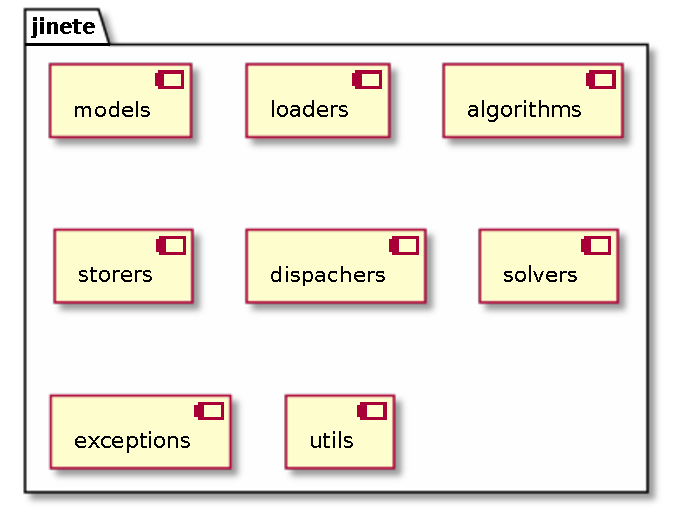
\includegraphics[width=0.5\textwidth]{modules-overview}
            \caption{Diagrama basado en módulos de la biblioteca \texttt{jinete}}
            \label{img:modules_overview}
          \end{figure}

          \paragraph{}
          En cuanto a la organización completa de la biblioteca, esta se divide en 4 módulos principales, que además de apoyarse entre si, utilizan otros módulos de menor tamaño tal y como se comentará a lo largo del apartado. En la \cref{img:modules_overview} se incluye una representación gráfica de estos. En cuanto a los módulos principales, a continuación se proporciona una breve descripción acerca de cada uno de ellos (el orden en que se describen se corresponde con el flujo natural en que estos se interrelacionan lo cual pretende servir para clarificar aún más su funcionamiento):

          \begin{itemize}
              \item \texttt{models}: Es el encargado de definir las entidades que representan los distintos elementos necesarios para modelar los distintos problemas de rutas, entre los que se encuentran clases como \texttt{Vehicle}, \texttt{Route} o \texttt{Stop}. Dichas entidades son las encargadas de poseer la información acerca de las restricciones del problema (como por ejemplo la ventana temporal en que es factible llevar a cabo parada de recogida para un determinado viaje), pero además se encargan de recoger el estado tras cada etapa de ejecución del proceso de optimización (como por ejemplo el instante de tiempo en que se encuentra un determinado vehículo al haber realizado un secuencia concreta de viajes).Dichas entidades representan además un \say{contrato} entre el resto de módulos y submódulos de la biblioteca, lo cual es una de las herramientas que permite hacer más mantenible y ampliable la implementación realizada. Posteriormente se detalla de manera más precisa, pero a modo de ejemplo es fácil apreciar las ventajas de definir una entidad común \texttt{Route} que pueda ser utilizada por las distintas estrategias de optimización sin que estas requieran de otra característica adicional, lo que permite flexibilizar la capacidad de combinación y/o composición de dichas estrategias. En el \cref{sec:implementation_components_data_model} se lleva a cabo una descripción más detallada acerca del módulo.

              \item \texttt{loaders}: Tal y como se ha comentado anteriormente a modo de ejemplo, la responsabilidad de este módulo consiste en ser capaz de cargar los datos desde una fuente de datos externa sobre la cual estos están definidos siguiendo un determinado formado posiblemente distinto del deseado, el cual consiste en las definidas por el módulo \texttt{models}. De esta manera, es posible aplicar indistintamente las distintas técnicas y herramientas implementadas en la biblioteca ignorando la estructura de los datos originales. Más adelante se describe de manera más detallada, sin embargo es interesante remarcar que en dicha tarea hay dos dimensiones principales: la \say{lectura} de la fuente de datos, la cual puede ser desde la carga de un fichero hasta el acceso a una base de datos o la realización de una petición \texttt{HTTP} a un sistema externo, del \say{procesamiento} del propio formato de los datos, que puede ser el definido por distintos autores o sistemas externos.En el \cref{sec:implementation_components_data_loading} se lleva a cabo una descripción más detallada acerca del módulo.

              \item \texttt{algorithms}: La responsabilidad de este módulo consiste en alojar las herramientas necesarias para poder llevar a cabo el proceso de optimización del problema en cuestión. Es decir, es quien contiene la implementación tanto de los algoritmos heurísticos tales como asignación voraz o búsqueda local, así como las metaheurísticas que se encargan de coordinar su ejecución. Además, contiene la lógica necesaria para ser capaz de resolver el problema a través de solvers externos de optimización lineal (métodos exactos). El modo de funcionamiento de estos algoritmos consiste en \say{rellenar} o \say{modificar} el estado de distintas entidades como \texttt{Route} o \texttt{Stop}, de tal manera que el formato siga siendo consiste para que puedan seguir siendo utilizadas tanto durante otras etapas del proceso de optimización como por el correspondiente módulo encargado de exportar dichos resultados. En el \cref{sec:implementation_components_optimization} se lleva a cabo una descripción más detallada acerca del módulo.

              \item \texttt{storers}: Es el módulo encargado de almacenar los resultados obtenidos tras el proceso de optimización. este espera recibir una planificación compuesta por uno o más vehículos, la cual almacena de distintas formas según sea la entidad concreta elegida para el proceso. Nótese que en este caso el término \say{almacenar} se utiliza en un sentido más amplio, ya que se refiere tanto al proceso de almacenar los resultados en un medio persistente como un fichero o una base de datos, como al proceso de mostrar un informe detallado en la terminal de salida o mostrar una representación gráfica de las rutas construidas. En el \cref{sec:implementation_components_exportation} se lleva a cabo una descripción más detallada acerca del módulo.


          \end{itemize}

          \paragraph{}
          Además de los módulos descritos anteriormente, la biblioteca implementada (\texttt{jinete}) incluye otros módulos de menor relevancia, pero igualmente importantes para el correcto funcionamiento de la misma. A continuación se incluye una breve descripción acerca de estos:

          \begin{itemize}

              \item \texttt{dispachers}: La labor que desempecha este módulo consiste en orquestar la comunicación entre \texttt{loaders}, \texttt{models} y \texttt{storers}. Como es natural, la estrategia más sencilla consiste en la comunicación unidireccional que carga una instancia del problema, aplica el proceso de optimización y después exporta los resultados en un medio persistente. Sin embargo, con la extensión de este módulo es posible llevar a cabo otras estrategias que permitan procesos de planificación en tiempo real entre otros.

            \item \texttt{solvers}: La responsabilidad que desempeña es la de simplificar el proceso de instanciación necesario para proceder con la optimización. El motivo es que para la mayoría de situaciones, no es neceario llegar a un nivel elevado de detalle para poder utilizar la biblioteca, por lo que este módulo se encarga de simplificar al máximo el proceso.

            \item \texttt{exceptions}: Contiene la definición acerca de las distintas situaciones de error que pueden darse durante el proceso de ejecución de la biblioteca, que después son comunicados a través de excepciones al usuario de la misma.

            \item \texttt{utils}: Se encarga de definir todas aquellas herramientas necesarias para el correcto funcionamiento de la biblioteca pero que no necesariamente se refieren al contexto de optimización combinatoria, tales como estructuras de datos o funciones auxiliares.

          \end{itemize}

          \paragraph{}
          Una vez se ha llevado a cabo una descripción acerca de todos los módulos que forman la implementación realizada, en los siguientes apartados se procede a profundizar con un mayor grado de detalle en los más relevantes, entre los que se encuentran el modelo de datos utilizado, el proceso de carga de instancias, la optimización de la instancia del problema y finalmente, el proceso de almacenamiento de resultados. Por el contexto del trabajo, se presta especial detalle a los apartados del modelado y resolución del problema, indicando más brevemente los procesos de carga y almacenamiento de datos.

        \subsubsection{Modelo de Datos}
        \label{sec:implementation_components_data_model}

          \paragraph{}
          Para poder resolver en condiciones adecuadas un problema de optimización combinatoria tan complejo como el \emph{Dial-a-Ride}, donde es necesario tener en cuenta una gran cantidad de situaciones, y a su vez, entender cómo han sido alcanzadas, un buen punto de partida es el de aclarar y uniformizar los conceptos que después serán utilizados por los métodos de resolución. En este caso, el punto de partida para llevar a cabo dicho proceso consiste en las entidades ya definidas previamente, en el \cref{sec:formulation_keywords} donde se comentaron todos muchos de los terminos y palabras clave utilizadas para comentar el problema. Dichas definiciones han servido como punto de partida para definir las entidades de datos utilizadas a lo largo de la implementación realizada, las cuales en su gran mayoría se relacionan de manera biyectiva. Por lo tanto, el resto del apartado se dedica a indicar brevemente dicha adaptación de los conceptos en entidades de datos a la vez que se describe como estas se relacionan entre si. Además, en la \cref{img:data_model_overview} se incluye un diagrama que ilustra la descripción que se llevará a cabo a continuación.

          \begin{figure}[!ht]
            \centering
            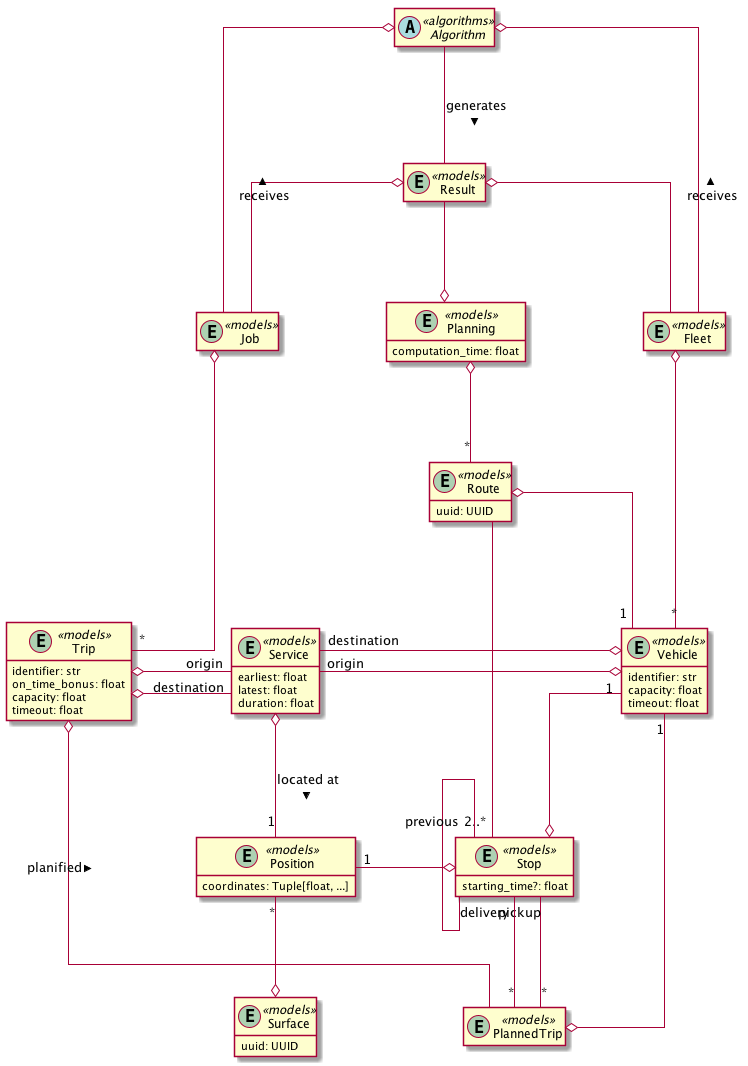
\includegraphics[width=0.9\textwidth,height=0.9\textheight,keepaspectratio]{data-model-overview}
            \caption{Modelo de datos simplificado de la biblioteca \texttt{jinete}.}
            \label{img:data_model_overview}
          \end{figure}

          \paragraph{}
          Siguiendo el mismo orden que el llevado a cabo en el \cref{sec:formulation_keywords}, la primera entidad a comentar es \texttt{Position}, que como su propio nombre indica, se trat de la estructura de datos encargada de modelizar una posición en el espacio. Esto es, aquella que almacena las coordenadas que \say{apuntan} a un determinado punto del espacio. Como es natural, esta es utilizada por el resto de entidades con necesidades de ser localizables en el espacio. En este caso se corresponden con \texttt{Service} (actividad de recogida o entrega relacionada con un viaje) y \texttt{Stop} (acción de moverse hacia un determinado lugar llevada a cabo por un vehículo). Además, para mantener en un contenedor común todas las posiciones surge la entidad \texttt{Surface}.

          \paragraph{}
          La entidad \texttt{Surface} es la encargada de almacenar, proveer e interactuar con entidades \texttt{Position}. Es decir, es la encargada de realizar los cálculos de distancias entre distintos puntos del espacio. Por tanto, tiene la responsabilidad de definir la métrica utilizada en caso de que la distancias sean aritméticas (\emph{Euclídea}, \emph{Manhattan}, etc.) o de calcularlas apoyándose en un servicio cartográfico externo entre otros.

          \paragraph{}
          Siguiendo con las entidades que se encargan de definir las restricciones del problema (posteriormente se continúa con aquellas que recogen el estado y por tanto, el resultado de la optimización) es necesario comentar la labor que desempeña \texttt{Service}. Tal y como se ha dicho anteriormente, esta representa el requisito de llevar a cabo una determinada acción en una determinada posición del espacio. Es decir, es quien contiene información acerca de la ventana temporal disponible para visitar una determinada posición por un vehículo. Además, ofrece la posibilidad de indicar la duración requerida de dicho servicio. Esto es útil para modelar los tiempos de carga y descarga correspondientes. Sin embargo, \texttt{Service} no se utiliza únicamente para representar las tareas de carga y descarga de los viajes. Además, es utilizada para representar el concepto de tiempo de las ventanas temporales de inicio y fin de los vehículos. Es decir, es la manera de representar que un vehículo puede comenzar a operar durante un cierto intervalo de tiempo, y puede volver al almacén en otro determinado intervalo de tiempo. En caso de que ambos puntos sean el mismo, nótese que si dichas ventanas temporales (de comienzo y fin) son disjuntas entonces dicho vehículo estaría obligado a realizar al menos un viaje (lo que puede generar situaciones de infactibilidad de la solución del problema si no hay suficientes viajes disponibles).

          \paragraph{}
          Una de las entidades más importantes desde el punto de vista de la formulación del problema es \texttt{Trip}. Esta es la encargada de \say{conectar} los servicios de recogida y entrega entre si, de tal forma que no puedan ser realizados indistintamente o de manera parcial. Es decir, es quien impone la restricción de que primero se ha de realizar la tarea de visita y, en un tiempo no superior a la duración máxima de viaje, se debe realizar la entrega. Posteriormente, cuando se lleve a cabo la descripción de la entidad \texttt{Stop} se expondrá de manera más detallada cómo es el proceso para llevar esto a cabo. Además de lo indicado, esta es la entidad encargada de indicar la cantidad de espacio (carga) requerido en el vehículo.

          \paragraph{}
          La siguiente entidad a remarcar consiste en \texttt{Job}, cuyo cometido es actuar como un contenedor de viajes (objetos \texttt{Trip}) de tal manera que puedan ser consultados de manera sencilla por otras entidades del modelo de datos. En este caso, \texttt{Job} se corresponde con una visión estática del problema, es decir, no posee ningún conocimiento sobre qué viajes han sido realizados y cuáles no (dicha tarea es responsabilidad de otras entidades).Además de contener todos los viajes del problema, esta también se encarga de contener la entidad \texttt{Objective}, la cual se encarga de representar la función objetivo a optimizar. Esta puede ser de naturaleza muy variada dependiendo de la versión concreta del problema de rutas a resolver. En este trabajo, la más utilizada es la del problema \emph{Dial-a-Ride} por razones obvias, la cual trata de minimizar la distancia total llevada a cabo por los vehículos disponibles.

          \paragraph{}
          Dejando de lado la representación de las necesidades a satisfacer, el siguiente paso es comentar los recursos disponibles para llevarlas a cabo. Como en todos los problemas de rutas, la entidad fundamental que actúa como recurso disponible es la del vehículo. En nuestro caso, dicha función la desempeña \texttt{Vehicle}. En este punto, hay una decisión de diseño importante a tomar, que consiste en la elección entre: \begin{enumerate*}[label=(\alph*)] \item utilizar la entidad vehículo para representar tanto las restricciones que este presenta (tales como capacidad máxima, tiempo máximo de ruta, etc.) como el estado actual (secuencia de tareas o viajes completados, tiempo actual, capacidad actual, etc.) o, por contra, \item dividir dicha entidad en dos, siendo una de ellas la encargada de representar las restricciones anteriormente citadas y otra la encargada de almacenar el estado actual \end{enumerate*}. Como es obvio, cada una una de estas alternativas posee distintas ventajas y desventajas, siendo la primera de ellas más simple pero menos versátil y la segunda, a costa de un mayor grado de complejidad, permite abstraer mejor los conceptos facilitando la implementación de estrategias de optimización avanzadas que requieran de mantener distintas versiones de un mismo vehículo de manera simultanea minimizando la duplicidad de información (y los posibles errores que puedan derivar de dicha situación). En este caso, se ha escogido la segunda opción, por lo que la entidad \texttt{Vehicle} es encargada únicamente de modelizar las restricciones de un vehículo sin mantener constancia de su estado.


          \paragraph{}
          Al igual que se ha indicado para el caso de \texttt{Position} y \texttt{Job}, es necesario añadir una entidad adiccional que actúe como contenedor de estas, siendo \texttt{Surface} y \texttt{Job} respectivamente en los anteriores casos. Por lo tanto, el contenedor de endidades \texttt{Vehicle} se ha denominado \texttt{Fleet} y, al igual que ocurre con \texttt{Job}, su único cometido consiste en proveer de las correspondientes entidades a quien lo requiera. Nótese que el problema \emph{Dial-a-Ride} asume una cantidad finita de vehículos, por lo que esto deberá ser acorde con el funcionamient de \texttt{Fleet}. Sin embargo, existen otros problemas como el \emph{Pickup and Delivery Problem} en que no hay una cota máxima del número de vehículos (a costa de que todos sean iguales entre sí).

          \paragraph{}
          Una vez comentado el significado de todas las entidades de naturaleza estáticas del modelo de datos, el siguiente paso es proceder al razonamiento de las entidades dinámicas, encargadas de almacenar el estado de la optimización. Estas se caracterizan por estar construidas apoyándose en gran medida sobre las anteriores, además de presentar un mayor grado de dificultad tanto en su implementación como explicación por su naturaleza cambiante.

          \paragraph{}
          Siguiendo el orden del \cref{sec:formulation_keywords}, la siguiente entidad a comentar es \texttt{Stop}, cuya función principal es la de representar la realización de un determinado servicio, por un determinado vehículo un estado concreto (posteriormente se indicará cómo se lleva a cabo dicha representación del estado). La entidad \texttt{Stop} se relaciona con el resto de la siguiente manera: con la entidad \texttt{Vehicle} a la cual se refiere, con la entidad \texttt{Position} sobre la cual se localiza, con la entidad \texttt{PlannedTrip} (que se comenta más adelante) sobre la cuál es capaz de relacionarse tanto con el viaje y los servicios requeridos, como con la parada relacionada (de entrega futura si esta es de recogia, o de recogida previa si esta es de entrega). De esta manera es posible verificar si el viaje completo se ha llevado a cabo desde una de las paradas, que no necesariamente tienen por qué ser contiguas entre sí. Adiccionalmente, la entidad \texttt{Stop} incluye otra relación adiccional consigo misma, que representa la anterior parada. De esta manera, todas las paradas de un mismo vehículo están relacionadas entre sí como una lista enlazada. La ventaja de este enfoque es que los cálculos tanto de tiempo como de capacidad actuales, pueden ser calculados desde la propia entidad \texttt{Stop} y la versión anterior de esta generandose una \emph{relación de recurrencia de primer orden}. Por último, esta entidad se relaciona con \texttt{Route}, que como veremos más adelante actúa como contenedor de paradas.

          \paragraph{}
          La siguiente entidad a comentar es \texttt{PlannedTrip}, que como su propio nombre indica se refiere a la realización de un viaje. Esta entidad guarda una \emph{relación fuerte} con las dos paradas necesarias para completar el viaje (la de recogida y la de entrega). Además, esta relacionada con la entidad \texttt{Vehicle} correspondiente.

          \paragraph{}
          Anteriormente se ha indicado que la decisión tomada acerca de cómo representar las restricciones fijas de los vehículos así como su estado actual ha consistido en dividirlo en dos entidades. Ya hemos descrito \texttt{Vehicle}, que es la responsable de definir las restricciones. Sin embargo, todavía no hemos indicado cómo se almacena el estado. Para ello, se ha decidido utilizar la entidad \texttt{Route}, cuyo cometido es almacenar la secuencia de paradas (entidades \texttt{Stop}), y a su vez mantener una relación a través de la cual sea posible recuperar las restricciones de la misma (\texttt{Vehicle}). La ventaja que esta estrategia presenta consiste en la \say{facilidad} para poder mantener varias instancias de la entidad \texttt{Route} referidas al mismo vehículo y al mismo tiempo para que las comparaciones entre estas (para elegir la más beneficiosa para el resultado final) sean mucho más sencillas. Esto es un factor importante en la resolución de este tipo de problemas donde la carga computacional derivada de la evaluación combinatoria es muy elevada.

          \paragraph{}
          Antes de finalizar, es necesario comentar en qué consiste la entidad \texttt{Planning}, la cuál actúa como un contenedor de entidades \texttt{Route}. Tal y como se ha comentado antes, estas se refieren a la secuencia de paradas para cada vehículo. Nótese que deben satisfacer la restricción de que  un vehículo tan solo tenga una ruta a realizar por razones obvias. Por último, se añade una entidad más denominada \texttt{Result}, que se encarga de poner en común la flota de vehículos, el conjunto de viajes a realizar, y la asignación generada mediante las entidades \texttt{Fleet}, \texttt{Job} y \texttt{Planning} respectivamente. Lo interesante de esta entidad es que es la utilizada como valor de entrada y salida para muchos de los métodos de resolución implementados (entidades \texttt{Algorithm}), lo cual permite que estos puedan ser intercambiados y combinados entre sí fácilmente.

          \paragraph{}
          Tal y como se puede apreciar a lo largo del apartado, el modelado del problema de manera adecuada se ha correspondido con una tarea de gran peso para la implementación realizada. A lo largo de la descripción, se ha tratado de comentar la taxonomia definida manteniendo el equilibrio adecuado entre detalle y extensión del mismo, dejando de lado algunos detalles técnicos de menor relevancia para la visión general del modelo de datos.

        \subsubsection{Carga de Datos}
        \label{sec:implementation_components_data_loading}

          \paragraph{}
          El proceso de carga de datos en la implementación llevada a cabo consiste más concretamente en la lectura de los valores concretos que definen las diferentes instancias del problema a resolver, los cuales consisten en el número de viajes requeridos así como las características concretas de cada uno de ellos, o los vehículos disponibles para satisfacer dichos viajes, con sus corresponientes limitaciones tanto de tiempo como de carga. Este apartado se dedica a describir cómo es llevado a cabo dicho proceso desde la perspectiva del flujo de los datos, es decir, desde que se realiza la llamada que comienza el proceso de carga, hasta que están construidos por completo los elementos necesarios para llevar a cabo el proceso de optimización.

          \begin{figure}[!ht]
            \centering
            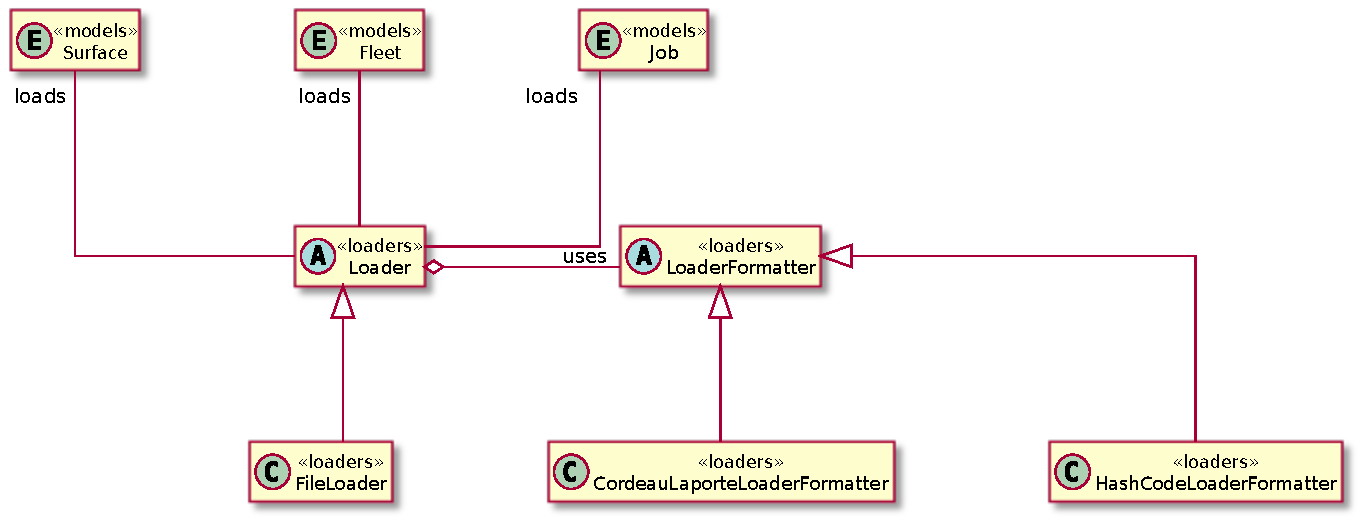
\includegraphics[width=0.9\textwidth,height=0.9\textheight,keepaspectratio]{loaders-overview}
            \caption{Diagrama de clases del módulo \texttt{loaders} perteneciente a la biblioteca \texttt{jinete}.}
            \label{img:loaders_overview}
          \end{figure}

          \paragraph{}
          Tal y como se ha comentado anteriormente, el módulo destinado a dicha tarea se ha denominado \texttt{loaders}. En este se ha definido una interfaz \texttt{Loader}, la cual sirva para definir la estructura que deben tener todas las implementaciones destinadas a la carga de datos. Esta proporciona acceso a las correspondientes instancias \texttt{Surface}, \texttt{Fleet} y \texttt{Job} que definen el espacio geométrico, la flota de vehículos y los viajes a realizar respectivamente, tal y como se indicó en el anterior apartado. El modo en que se ha definido dicha interfaz permite que esta pueda cargar los datos de manera \emph{lazy} (o bajo demanda), es decir, que la carga no se lleve a cabo hasta el momento inmediatamente anterior a su utilización.

          \paragraph{}
          La idea sobre la interfaz \texttt{Loader} es que las entidades que la implementen se encargen de proveer de acceso a los datos en crudo, pero sin profundizar en el formato de estos. Actualmente, se ha llevado a cabo la implementación \texttt{FileLoader}, que se encarga de cargar el contenido de un fichero. Una extensión natural podría ser la de implementar un \texttt{URLLoader} que se encargase de cargar el contenido alojado en una dirección web. Sin embargo, ninguna de estas implementaciones tiene la responsabilidad de \say{entender} el formato de estos datos y transformarlos en las entidades anteriormente citadas. Para ello se ha definido el concepto de \texttt{LoaderFormatter}, cuyo objetivo es el de construir las correspondientes entidades a partir de los datos. En este caso, la implementación principal es la de \texttt{CordeauLaporteLoaderFormatter}, que se encarga de generar las corespondientes instancias a partir del formato de definición de las instancias del problema definido por Cordeau y Laporte para las instancias usadas como \emph{Benchmark} en \cite{cordeau2003tabu}. El diagrama de clases que ilustra la manera en que se interrelacionan las clases definidas en el módulo \texttt{loaders} se incluye en la \cref{img:loaders_overview}.

          \paragraph{}
          A modo de ejemplo, a continuacion se comenta la secuencia de acciones que son llevadas a cabo para la carga de datos utilizando la implementación \texttt{CordeauLaporteLoaderFormatter}. Como ejemplificación acerca del formato en cuestión, a través del siguiente enlace se puede consultar la instancia \texttt{a2-16.txt} utilizada en el benchmark del paper anteriormente citado: \url{http://fc.isima.fr/~lacomme/Maxime/ELSapproachDARP/instances/a2-16.txt}. En la primera línea se incluyen el número de vehículos disponibles, el número de paradas a satisfacer (incluyendo recogida y entrega, por lo que el número de viajes es la mitad), el tiempo máximo de viaje por vehículo, el número de viajes que pueden compartir un vehículo de manera simultánea y la duracción máxima de viaje (contabilizado desde que se deja el punto de recogida hasta que se alcanza el punto de entrega, es decir, únicamente es contabilizado el tiempo de trayecto para esta restricción). Seguidamente se incluye una secuencia con todas las paradas a satisfacer, donde la primera mitad se refiere a las recogidas mientras que la segunda mitad representa las entregas. Por tanto, suponiendo $n$ viajes, la parada $i$ representa la recogida y la parada $i + n$ la entrega (por lo que, como es obvio, existen $2n$ paradas). Cada parada se define de la siguiente forma: un identificador de parada, las coordenadas del punto donde satisfacer la parada. En este caso, están definidas sobre un espacio euclídeo bidimensional por lo que las distancias son calculada aplicando la norma dos (o $d(x, y) = \sqrt{(x_{1} - y_{1}) ^ 2 + (x_{2} - y_{2}) ^ 2}$). Seguidamente, se indica la duracción del tiempo de carga/descarga. A continuación, se incluye la capacidad requerida por el viaje. Nótese que esta es opuesta en la recogida y entrega, siendo la primera positiva y la segunda negativa. Esto facilita la integración de la instancia en formulaciones como problema de programación lineal. Finalmente se incluyen las ventanas temporales en que satisfacer cada parada. En este caso, algunas de ellas son abiertas y otras cerradas, dependiendo de si el viaje es de tipo \emph{inbound} (recoger en un intervalo prefijado) u \emph{outbound} (entregar en un intervalo prefijado).

          \paragraph{}
          Una vez comentado el formato de entrada, el siguiente paso es entender cómo este es transformado en las entidades definidas en el modelo de datos. El primer paso es la construcción del espacio geométrico, es decir, la instancia \texttt{Surface}. Esta es común entre la flota de vehículos y el conjunto de viajes a realizar por lo que es necesario que sea el primer elemento a construir. Dicha implementación incluye un método \verb|get_or_create_position(coordinates: Tuple[float]) -> Position| por lo que el proceso es muy sencillo al no requerir de una lectura inicial de todas las coordenadas. A continuación se construye la secuencia de vehículos, la cual requiere únicamente de la primera línea del fichero de datos, creando posteriormente la instancia \texttt{Fleet}. Finalmente, se procede a la creacción de la entidad \texttt{Job}, compuesta por el conjunto de viajes (o instancias \texttt{Trip}). Para construir estas se procede a la iteracción de las restantes filas siguiendo el enfoque indicado anteriormente $(i, i+n)$ para enlazar tanto la parada de recogida como la de entrega. Una vez construidas las correspondientes instancias de \texttt{Surface}, \texttt{Fleet} y \texttt{Job} ya se está en condiciones necesarias para proceder a la fase de optimización del problema, la cual se describe en el siguiente apartado.

        \subsubsection{Optimización del Problema}
        \label{sec:implementation_components_optimization}

          \paragraph{}
          El módulo \texttt{algorithms} representa una de las partes más interesentas (a la vez que críticas) de la implementación llevada a cabo. La lógica que implementa es la encarga de llevar a cabo la resolución de problemas en la biblioteca \texttt{jinete} por lo que la explicación acerca de cómo esta funciona es especialmente interesante. Tal y como se ha indicado previamente a lo largo del apartado dedicado a la descripción de la carga de datos, responsabilidad del módulo \texttt{loaders}, en el cual se ha definido una interfaz denominada \texttt{Loader}, en este caso se ha hecho lo correspondiente definiendo la interfaz \texttt{Algorithm}. Dicha interfaz espera recibir como entidades de entrada una instancia \texttt{Fleet} y otra \texttt{Job}, que representan las características de la flota de vehículos y el conjunto de viajes a realizar respectivamente. Nótese que en este caso no se requiere de una instancia \texttt{Surface}, lo cual es debido a que esta viene dada de manera implícita sobre las posiciones (\texttt{Position}) que componen el resto de entidades. Para proceder con la ejecución, la interfaz \texttt{Algorithm} ofrece un método \verb|optimize() -> Result|, que como resultado genera una nueva entidad \texttt{Result}, la cual contiene la planificación generada para la flota de vehículos y conjunto de viajes dados. Esto se comenta de manera más detallada en el apartado dedicado al almacenamiento de resultados, lo cual es responsabilidad del módulo \texttt{storers}.

          \begin{figure}[!ht]
            \centering
            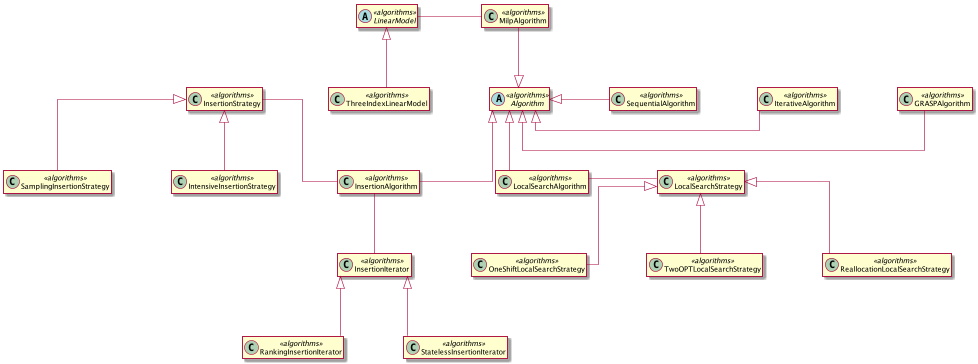
\includegraphics[width=0.9\textwidth,height=0.9\textheight,keepaspectratio]{algorithms-overview}
            \caption{Diagrama de clases del módulo \texttt{algorithms} perteneciente a la biblioteca \texttt{jinete}.}
            \label{img:algorithms_overview}
          \end{figure}

          \paragraph{}
          Una vez entendido el modo de funcionamiento definido por la interfaz \texttt{Algorithm}, es posible dejar de lado la manera en que se intercomunican las distintas implementaciones, tanto entre sí como con otras entidades externas para poder enfocar la descripción en la funcionalidad que desempeñan cada una de ellas. Para tratar de simplificar el razonamiento acerca de cómo se relacionan, en la \cref{img:algorithms_overview} se incluye el diagrama de clases del módulo \texttt{algorithms}. Sin embargo, este no proporciona una descripción acerca de la función que desempeña cada una de las subimplementaciones más allá del nombre que estas tienen. Por lo tanto, a continuación se proporciona una descripción más detallada acerca de estas:

          \begin{itemize}

              \item \texttt{Algorithm}: Actúa como la interfaz que define la manera de utilizar las distintas subimplementaciones, tanto desde el punto de vista de los parámetros de entrada mínimos (dependiendo de la subimplementación estas pueden requerir ciertos parámetros opcionales), como del valor obtenido tras su ejecución, la cual se lleva a cabo mediante la llamada al método \texttt{optimize()} tal y como se indicó previamente.

              \item \texttt{InsertionAlgorithm}: La funcionalidad que desempeña esta subimplementación consiste en insertar nuevos viajes a rutas previamente existentes, así como crearlas en caso de que el correspondiente vehículo se encontrase en un modo ocioso (sin haber sido utilizado hasta el momento). Para proceder a la inserción de nuevos viajes en las distintas rutas disponibles, es necesario definir la forma en que estos serán emparejados respectivamente. Para ello, lo primero es definir la manera de recorrer todas estas combinaciones disponibles, que dependiendo del tamaño del problema y la configuración llevada a cabo, pueden llegar a ser inabarcables. Puesto que el algoritmo de inserción funciona de manera iterativa tratando de añadir todos los viajes que pueda mientras sea posible, parece interesante definir la manera en que iterar los pares \texttt{(Route, PlannedTrip)}. En este caso es importante remarcar que las combinaciones han de llevarse a cabo sobre viajes planeados, de tal forma que se tenga en cuenta el hueco en que se pretenden insertas las correspondientes paradas de recogida y entrega. Esto es debido a que dicho factor afectará de alguna forma tanto al coste como al estado resultante de la ruta (de ahí que el número de casos a evaluar se convierta en elevado). Como es natural, la iteración de estos pares se lleva a cabo de tal manera que primero se comprueben aquellos cuya valoración (o beneficio) sea mayor según el criterio correspondinte:

                  \begin{itemize}

                      \item \texttt{RouteCriterion}: Se compone por una clase abstracta que espera recibir como entrada la dirección de optimización (maximización o minimización) y expone métodos de ordenación y cálculo de los $k$ mejores. Para poder aprovecharse de estos es necesario implementar el método \texttt|scoring(route: Route) -> float|, que se encarga de calcular la puntuación de una determinada ruta.

                      \item \texttt{EarliestLastDepartureTimeRouteCriterion}: Se trata de un criterio de minimización y calcula la puntuación de la ruta como el tiempo final de la ruta. Por tanto, se valora más positivamente la ruta que antes haya terminado.

                      \item \texttt{ShortestAveragePlannerTripDurationCriterion}: Se trata de un criterio basado en minimización y la puntuación es calculada como el promedio de la duración de cada viaje de la ruta. Es decir, la diferencia de tiempos entre entrega y recogida.

                      \item \texttt{ShortestTimeRouteCriterion}: Es un criterio de minimización del tiempo de ruta. Es decir, el tiempo que pasa desde que el vehículo sale del almacén hasta que este regresa.

                      \item \texttt{LongestTimeRouteCriterion}: Es un criterio de maximización del tiempo de ruta. Es decir, es el opuesto del anterior y la intuición que este presenta es la de tratar de aprovechar al máximo el vehículo escogido.

                      \item \texttt{LongestUtilTimeRouteCriterion}: Se trata de un criterio de maximización que contabiliza la distancia recorrida por el vehículo con carga. La intuición tras este criterio consiste en reducir el tiempo en que el vehículo viaja vacío.

                  \end{itemize}

                  Una vez comentadas las distintas alternativas disponibles para valorar una ruta, el siguiente paso es definir los modos en que puede iterarse a través de la secuencia generada por dicho orden.

                  \begin{itemize}

                      \item \texttt{InsertionIterator}: Define la interfaz de iteración de las rutas recibiendo como entrada tanto el conjunto de rutas como el criterio de valoración a utilizar.

                      \item \texttt{RankingInsertionIterator}: Mantiene un estado interno a lo largo de la ejecución del algoritmo de insercción, de tal manera que tras cada cambio de estado se recalculan únicamente las valoraciones que hayan sufrido cambios para posteriormente ser reordenadas. Puesto que el número de pares puede crecer de manera exponencial, existe la posibilidad de generar un ranking truncado donde se eligen aleatoriamente $k < n$ viajes donde $n$ representa el número total de viajes, para después ir añadiendo cada vez un nuevo viaje de entre los $n-k$ restantes. De esta manera es posible controlar la eficiencia computacional de la implementación a costa de obtener resultados ligeramente peores.

                      \item \texttt{StatelessInsertionIterator}: Se trata de una versión que no mantiene el estado. Tras cada nueva iteración recalcula la valoración para todos los pares de rutas y viajes planificados, escogiendo el que minimice (o maximice) el criterio escogido.

                  \end{itemize}

                  Una vez que se ha definido tanto el criterio de valoración de las rutas como la forma de iterar sobre los pares ya solo queda una pieza para poder completar la descripción del algoritmo de insección, la cuál es la propia estrategia de inserción. En este caso, el concepto de estrategia se refiere a la forma en que es posible insertar nuevos viajes en las rutas y como se ha comentado anteriormente, existen distintas alternativas:

                  \begin{itemize}

                      \item \texttt{InsertionStrategy}: Define la interfaz de insercción, la cual consiste en un método \verb|compute(route: Route, trip: Trip) -> List[Route]| donde el resultado es una lista de rutas generadas a partir de la enviada como parámetro, solo que con el nuevo viaje añadido.

                      \item \texttt{IntensiveInsertionStrategy}: La estrategia intensiva consiste en probar todos los pares $(i, j)$ posibles para insertar las paradas de recogida y entrega sobre la secuencia de paradas ya existentes. Esta estrategia es la que mejores resultados presenta, sin embargo, el número de rutas a evaluar puede ascender a $m \cdot log(m)$ donde $m$ es el número de paradas de la ruta, en el \say{peor} caso.

                      \item \texttt{TailInsertionStrategy}: La estrategia de inserción de cola consiste en tratar de insertar el viaje al final de la ruta. En este caso tan solo se crea una nueva ruta por lo que, en términos de eficiencia computacional, es la mejor de todas. Sin embargo, en este caso no se aprovecha la posibilidad de \emph{compartir vehículo} por varios viajes de manera simultanea. Este método es interesante para generar soluciones iniciales de manera eficiente que después puedan ser mejoradas por otras (meta-)heurísticas más avanzadas.

                      \item \texttt{SamplingInsertionStrategy}: Para tratar de equilibrar la estrategia de inserción intensiva (de alto coste computacional pero buenos resultados) con la de cola (de reducido coste computacional pero generalmente resultados mucho peores), se ha incluye una estratgia basada en sampleo de un número determinado de pares $(i, j)$ a evaluar, de tal manera que la insercción sea sobre un espacio de búsqueda más amplio pero a la vez se mantenga asequible sobre problemas de gran tamaño.

                  \end{itemize}

              \item \texttt{LocalSearchAlgorithm}: Para la implementación de técnicas de búsqueda local en la biblioteca \texttt{jinete}, se ha llevado a cabo la implementación de este algoritmo. Para que pueda ser utilizado, este espera recibir además de los parámetros de flota y conjunto de viajes, una solución inicial creada previamente por otro de los algoritmos. Por ejemplo, el \texttt{InsertionAlgorithm} indicado anteriormente. En cuanto a la salida esperada, este genera una nueva instancia \texttt{Result}. En este caso, la instancia se genera llevando a cabo distintas variaciones sobre la recibida como parámetro de entrada. Una vez definida la forma en que funciona el algoritmo de búsqueda local, lo siguiente es comentar cuáles son las transformaciones que este puede llevar a cabo. Estas se definen como estrategias de búsqueda local las cuales se han implementado, al igual que otras partes de la biblioteca, mediante una intefaz que define la forma de uso, así como subimplementaciones que incluyen la lógica correspondiente. A continuación se lleva a cabo una descripción de estas:

                  \begin{itemize}

                      \item \texttt{LocalSearchStrategy}: Se corresponde con la interfaz que define cómo es posible utilizarlas. En este caso, el parámetro de entrada es una entidad \texttt{Result}, que a través de la implementación del método \verb|improve() -> Result| describe la forma en que se pueden crear distintas estrategias de búsqueda local.

                      \item \texttt{OneShiftLocalSearchStrategy}: Se trata de una estrategia de búsqueda local que se aplica a nivel de cada ruta. El modo de funcionamiento es el siguiente: trata de mover cada parada 1 posición hacia atrás respecto de la secuencia de paradas y hace el cambio permanente cuando se llega a una reducción de coste.

                      \item \texttt{TwoOPTLocalSearchStrategy}: Consiste en la implementación del método \emph{2-OPT} de búsqueda local, que como es natural, se implementa a nivel de ruta. Tal y como se ha indicado en el \cref{sec:solving_local_search}, esta trata de \say{deshacer nudos} en la ruta mediante inversión del orden de paradas del segmento $(i, j)$ donde $1 \leq i < j \leq m$ y $m$ representa el número total de paradas de la ruta. Sin embargo, esta estrategia no proporciona resultados muy beneficiosos en problemas como el \emph{Dial-a-Ride}.

                      \item \texttt{ReallocationLocalSearchStrategy}: Se trata de una estrategia de búsqueda local entre rutas, es decir, a nivel de planificación. Esta estrategia consiste en elegir un viaje asignado a un determinado vehículo y tratar de añadirlo en la ruta de otro. El cambio se hace efectivo si hay una reducción de coste.

                  \end{itemize}

              \item \texttt{SequentialAlgorithm}: Se trata de una subimplementación que actúa como envoltorio para otras. Tal y como se ha definido la interfaz \texttt{Algorithm} así como la forma en que esta es utilizada por otras entidades, la cual consiste en una única llamada a la subimplementación correspondiente, esta no permite la concatenación de distintos métodos de resolución de manera nativa. Es por ello que se ha creado este emboltorio, cuyo objetivo es el de suministrar dicha funcionalidad. A modo de ejemplo, la definición de un algoritmo secuencial sencillo puede consistir en dos pasos: \begin{enumerate*} \item la creación de una solución inicial a partir de \texttt{InsertionAlgorithm} y, la mejora de esta a partir de algún método de búsqueda local proporcionado por \texttt{LocalSearchAlgorithm} \end{enumerate*}. Entonces, la manera de llevar esto a cabo en la biblioteca \texttt{jinete} es a partir de \texttt{SequentialAlgorithm}.

              \item \texttt{IterativeAlgorithm}: Al igual que \texttt{SequentialAlgorithm} proporciona la funcionalidad de poder concatenar distintos algoritmos proporcionando un envoltorio, la manera de proporcionar iteratividad es a partir de \texttt{IterativeAlgorithm}. En este caso, el término \emph{iteratividad} se refiere a la ejecución repetida de un mismo algoritmo durante un número prefijado de veces, o una condición de parada dada, escogiendo la mejor solución en términos de coste de entre todas las obtenidas en cada ciclo de iteracción.

              \item \texttt{GRASPAlgorithm}: Consiste en la implementación básica de la metaheurística \emph{GRASP}, la cual se describe en detalle en el \cref{sec:solving_grasp}. Tal y como se puede apreciar, gracias a la implementación de todas las distintas \say{piezas} que componen esta metaheurística como componentes independientes que pueden ser compuestas entre sí, la implementación de la misma es extremadamente sencilla. En concreto, esta está formada por la combinación de una instancia \texttt{IterativeAlgorithm}, que repite la ejecución de un \texttt{SequentialAlgorithm} compuesto por los dos pasos anteriormente utilizados como ejemplo: \texttt{InsertionAlgorithm} y \texttt{LocalSearchAlgorithm}. Sin embargo, la ventaja de este enfoque de \say{construcción} de algoritmos no es únicamente la de permitir la implementación de la metaheurística \emph{GRASP} de una manera sencilla, si no las capacidades de reutilización que sus partes tienen para poder implementar metaheurísticas mucho más avanzadas en próximos pasos del proyecto.

              \item \texttt{MilpAlgorithm}: Se trata de la implementación que se comunica con los solvers de resolución de problemas de programación mixta lineal y entera. Al igual que el resto de implementaciones, esta recibe como parámetros las entidades \texttt{Fleet} y \texttt{Job} que representan la instancia concreta del problema y se encarga de generar la formulación lineal del mismo para después transmitirla al correspondiente solver externo. Para llevar a cabo el proceso de formulación, se apoya en la utilización del correspondiente modelo lineal:

                  \begin{itemize}

                      \item \texttt{LinearModel}: Define la interfaz definida para transformar las correspondientes entidades \texttt{Fleet} y \texttt{Job} en restricciones del problema a resolver, de tal manera que estas sean comprensibles por las dependencias externas que permiten su ejecución.

                      \item \texttt{ThreeIndexLinearModel}: Se trata de la implementación de la formulación definida sobre un modelo de 3 índices para el problema \emph{Dial-a-Ride}.

                  \end{itemize}

          \end{itemize}

          \paragraph{}
          A lo largo del apartado se ha llevado a cabo una descripción acerca de los distintos componentes definidos sobre la interfaz \texttt{Algorithm} en la biblioteca \texttt{jinete}. A través de dicha descripción se ha tratado de justificar la utilidad obtenida por un mayor grado de esfuerzo en el diseño del módulo, lo cual permite aumentar el grado de reutilización de los componentes de este. Por lo tanto, una vez descrita la manera en que los problemas de optimización son resuelto, el siguiente paso es comentar cómo se lleva a cabo el proceso de almacenamiento de los resultados obtenidos, para lo cual se destina el próximo apartado.

        \subsubsection{Exportación de Resultados}
        \label{sec:implementation_components_exportation}

          \paragraph{}
          Tal y como se ha comentado a lo largo del apartado anterior, el resultado de la ejecución de los métodos de resolución del problema, que toman como entrada las instancias \texttt{Surface}, \texttt{Fleet} y \texttt{Job} que definen el espacio geométrico, la flota de vehículos disponibles y el conjunto de viajes a realizar respectivamente y generan como salida una instancia de tipo \texttt{Result}, la cual contiene la correspondiente planificación (representada por una instancia \texttt{Planning} tal y como se indicó en el apartado dedicado al modelo de datos). Entonces, la funcionalidad que desempeña el módulo \texttt{storers}, en el cual se centra este apartado, consiste en el almacenamiento, visualización y/o exportación de los resultados de la optimización, dados como una instancia \texttt{Result}.

          \paragraph{}
          A pesar de la aparente redundancia entre las entidades \texttt{Result} y \texttt{Planning}, hacer la división entre ambas es una decisión relacionada con la necesidad de reducir la responsabilidad que tiene cada una de ellas en el modelo de datos. En concreto, la entidad \texttt{Planning} se encarga de actuar como un contenedor de rutas de vehículos (instancias \texttt{Route}), mientras que \texttt{Result} se encarga de \say{conectar} la definición de la instancia del problema, dada por la flota de vehículos (\texttt{Fleet}) y el conjunto de viajes (\texttt{Job}), con la realización concreta de una asignación (\texttt{Planning}) generada por el correspondiente método de resolución. Dicha conexión entre definición del problema y asignación obtenida es necesaria de manera conjunta, entre otras cosas, para las tareas de exportación de resultados.

          \paragraph{}
          Una vez llevada a cabo la diferenciación entre \texttt{Result} y \texttt{Planning}, el siguiente paso es describir el modo de funcionamiento del módulo \texttt{loaders} desde una perspectiva de alto nivel, para posteriormente aclarar los detalles más interesantes de este. En este caso, el enfoque seguido para la implementación ha sido similar al utilizado en los módulos \texttt{loaders} y \texttt{algorithms}, es decir, se define una interfaz que define el modo de utilización de las distintas implementaciones incluidas en el módulo para tratar de maximizar la reusabilidad entre sí.

          \paragraph{}
          La interfaz que define el modo de utilización del módulo se ha denominado \texttt{Storer}, que espera recibir como entrada una instancia \texttt{Result} e incluye un método \verb|store()| que inicia la ejecución. Además, al igual que ocurría en el caso de la carga de datos, en este caso también se ha añadido el concepto de \texttt{StorerFormatter}, cuyo cometido es el de definir el formato de los datos de salida, sobre el cual se apoyan las correspondientes implementaciones para formatear los resultados. En la \cref{img:storers_overview} se incluye una ilustración del diagrama de clases simplificado que representa el contenido del módulo.

          \begin{figure}[!ht]
            \centering
            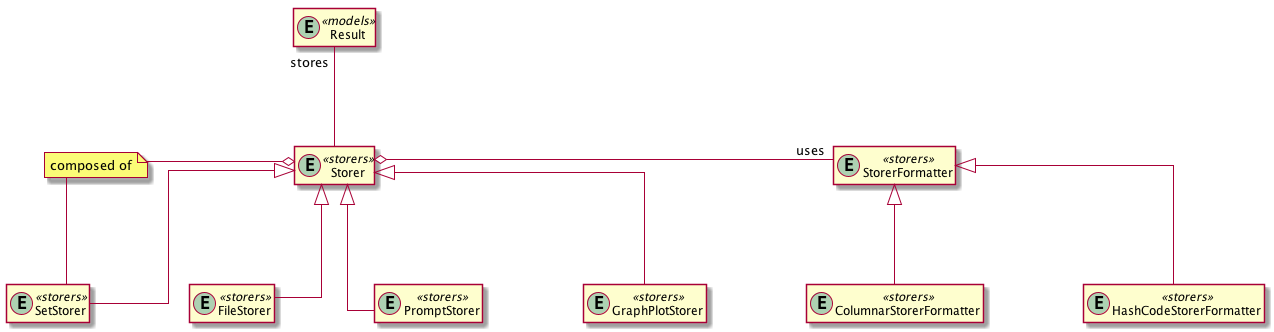
\includegraphics[width=0.9\textwidth,height=0.9\textheight,keepaspectratio]{storers-overview}
            \caption{Diagrama de clases del módulo \texttt{storers} perteneciente a la biblioteca \texttt{jinete}.}
            \label{img:storers_overview}
          \end{figure}

          \paragraph{}
          En cuanto a las implementaciones concretas de estas interfaz, en este caso se han incluido las siguientes:

          \begin{itemize}

            \item \texttt{PromptStorer}: El comportamiento que desempeña es el de mostrar por la salida estándar (línea de comandos) el resultado a almacenar, muy útil en tareas de desarrollo y validación.

            \item \texttt{FileStorer}: Se encarga de almacenar los resultados generados por el correspondiente \texttt{StorerFormatter} en una fichero del sistema lo cual proporciona persistencia para su posterior a otros sistemas.

            \item \texttt{GraphPlotStorer}: Se encarga de generar una representación en forma de grafo de la solución generada, el cuál muestra en una ventana independiente del sistema. Es posible configurarlo de tal manera que dicha representación sea exportada a un fichero en caso de que el sistema donde se ejecute la biblioteca no tenga capacidades gráficas.

            \item \texttt{StorerSet}: La utilidad de este \texttt{Storer} consiste en actuar como contenedor de otros. Puesto que la manera en que se ha definido la interfaz de utilización del módulo no permite la asignación de más de un \texttt{Storer} para una misma solución en el \texttt{Dispacher} secuencial, entonces es necesario crear una abstracción que permita obtener dicho comportamiento. En este caso, se ha llevado a cabo a través del \texttt{StorerSet}, que recibe como entrada un conjunto de implementaciones \texttt{Storer} y se encarga de propagar la llamada \verb|store()| a todos ellos con el mismo \texttt{Result}. De esta manera es posible por ejemplo, mostrar una representación gráfica del resultado obtenido, a la vez que se almacena en un fichero el resultado formateado.

          \end{itemize}

          \paragraph{}
          En cuanto a la manera de definir el formato de salida (cuando proceda), esto se lleva a cabo a través de la interfaz \texttt{StorerFormatter}, que se encarga de transformar una instancia \texttt{Result} en una cadena de caracteres. En la implementación actual se incluyen dos versiones:

          \begin{itemize}
            \item \texttt{ColumnarStorerFormatter}: Consiste en una versión en forma de columna que trata de incluir la mayor cantidad de información posible para poder entender el estado concreto de cada vehículo en cada punto concreto de la ejecución, muy útil sobre todo para tareas de análisis.

            \item \texttt{HashCodeStorerFormatter}: Consiste en un formato de salida muy simplificado y definido para una variación del problema \emph{Dial-a-Ride} utilizada como problema a resolver en una de las ediciones del concurso \emph{HashCode} llevado a cabo por la compañía \emph{Google}.

          \end{itemize}
          \paragraph{}
          Una vez finalizada la descripción acerca del modo de funcionamiento del módulo \texttt{storers} ya se puede tener una idea alto nivel acerca de cómo funciona la biblioteca implementada. En los futuros apartados se lleva a cabo un análisis acerca de los resultados obtenidos que demuestran la validez de la misma, así como su grado de eficiencia respecto de las soluciones óptimas obtenidas en trabajos de otros autores.

    \section{Resultados}
    \label{sec:results}

      \paragraph{}
      Tras haber llevado a cabo una descripción acerca de la implementación realizada, la cuál tal y como se ha indicado, consiste en una biblioteca desarrollada sobre el lenguaje \texttt{Python} cuyo nombre es \texttt{jinete}, el siguiente paso es comentar el procedimiento llevado a cabo para evaluar la validez y el correcto funcionamiento de la misma. Además, se espera que este apartado sirva como guía de uso de esta, incluyendo en todo momento las sentencias utilizadas tanto para iniciar la ejecución como para definir la configuración utilizada, de tal manera que el proceso sea totalmente reproducible si así se requiere.

      \paragraph{}
      El resto del apartado se organiza de la siguiente manera: en el \cref{sec:results_definition} se indica la manera en que se ha llevado a cabo el proceso de experimentación, indicando las instancias del problema \emph{Dial-a-Ride} escogidas para ello, la configuración exacta utilizada para la ejecución de la biblioteca y otros detalles como el tiempo máximo de ejecución. Seguidamente, en el \cref{sec:results_tables} se incluyen las tablas que muestran los resultados obtenidos tras la experimentación. Finalmente, en el \cref{sec:results_analysis} se lleva a cabo un análisis sobre dichos resultados, tratando de identificar ciertos patrones comunes así como posibles puntos de mejora.

      \subsection{Definición del experimento}
      \label{sec:results_definition}

        \paragraph{}
        Tal y como se ha indicado previamente, el objetivo de este apartado consiste en especificar cómo se ha llevado a cabo el proceso de obtención de resultados para demostrar la validez de la implementación realizada. Para ello, en primer lugar se indican los conjuntos de instancias utilizadas. Seguidamente se incluyen los scripts utilizados para comenzar la ejecución y finalmente se comentan otros factores como el tiempo máximo de ejecución para cada una de ellas (el cual es un factor a tener en cuenta en este tipo de problemas por razones obvias).

        \paragraph{}
        Las instancias utilizadas para el proceso de benchmarking o validación de resultados provienen de dos de los trabajos más populares relativos al problema \emph{Dial-a-Ride}. En primer lugar, se han utilizado las instancias creadas en \cite{cordeau2003tabu}, las cuales están compuestas por $20$ casos generados aleatoriamente y tienen tamaños desde los $3$ hasta los $10$ vehículos para satisfacer desde $24$ a $144$ viajes. Estás se identifican de la siguiente manera: \texttt{R1a.txt}, \dots, \texttt{R10a.txt}, \texttt{R1b.txt}, \dots,\texttt{R10b.txt}. El segundo trabajo del cual se han extraido las instancias utilizadas para el experimento es \cite{ropke2007models}, compuesto por dos grupos de $21$ casos cada uno, haciendo un total de $42$. Estas también han sido generadas de manera aleatoria, con tamaños desde $3$ vehículos y $16$ viajes hasta $8$ vehículos y $96$ viajes. En este caso las instancias se identifican de la siguiente forma: \texttt{a2-16.txt}, \dots, \texttt{a8-96.txt}, \texttt{b2-16.txt}, \dots,\texttt{b8-96.txt}. El motivo por el cual se han escogido estos dos grupos de instancias frente a otros ha sido la popularidad que tienen dentro del nicho de estudio del problema \emph{Dial-a-Ride}, habiendo sido utilizados en numerosos trabajos desde su publicación inicial.

        \paragraph{}
        En cuanto a cómo se ha llevado a cabo la ejecución desde la perspectiva de la utilización de la implementación llevada a cabo (\texttt{jinete}), en las \cref{code:launch,code:solve} se incluyen los fragmentos de código utilizados. Antes de empezar a comentar el objetivo de ambos, así como las sentencias más relevantes de cada uno de ellos, es necesario comentar los requisitos sobre el entorno de ejecución: En este sentido, el primer requisito es tener instalada una versión de \texttt{Python} mayor o igual a $3.7$ para que todas las dependencias funcionen correctamente. En cuanto a las dependencias dentro del lenguaje, en este caso tan solo es necesario instalar la última versión de la biblioteca implementada, la cuál se puede instalar a partir del código fuente. Sin embargo, al haberse desarrollado como una biblioteca open source, es tan sencillo como ejecutar el siguiente comando:

        \begin{minted}{bash}
          pip3 install jinete
        \end{minted}

        \paragraph{}
        Una vez configurado el entorno de ejecución ya se está en condiciones suficientes como para poder llevar a cabo la ejecución por lo que se procede a comentar la función que desempeña cada uno de los scripts.

        \paragraph{}
        El fragmento de código contenido en el fichero \texttt{launch.py}, que se muestra en la \cref{code:launch}, es el encargado de \say{orquestar} la ejecución del experimento. Es decir, es el encargo de llevar a cabo las ejecuciones concretas para cada instancia, encargandose de detectar cuando estas terminan para así lanzar la siguiente. Para hacer esto, se ha decidido que cada instancia sea ejecutada en un único proceso, permitiendo la ejecución de múltiples instancias al mismo tiempo si la máquina en cuestión es capaz de ello. En cuanto al contenido del fragmento de código, las líneas $15$ a $17$ son las encargadas de buscar los ficheros que contienen las definiciones de cada instancia y proceder a la ejecución en paralelo, las cuales son transmitidas a \texttt{ProcessPoolExecutor}, encargado de controlar el paralelismo actuando mediante un protocolo de cola definido como $1$ productor, $k$ consumidores donde $k$ es el número de procesadores de la máquina. Cuando llega el turno pertinente, la función \verb|run_one(file_path: Path)| es ejecutada, encargandose de llevar a cabo una llamada al comando \verb|python3 solve.py $FILE_PATH|. El resto de las sentencias son las encargadas de controlar los posibles errores, así como guardar los posibles mensajes de \texttt{logging} generados durante la ejecución.

        \begin{figure}[!hb]
    			\centering
    			\inputminted[frame=single,framesep=10pt,linenos]{python}{./code/launch.py}
    			\caption{Fragmento de código contenido en el fichero \texttt{launch.py}.}
    			\label{code:launch}
    		\end{figure}

        \paragraph{}
        Una vez comentado el fragmento de código encargado de llevar a cabo el proceso de control y lanzamiento de todas las instancias incluidas en el experimento, lo siguiente es comentar el segundo fragmento de código: Este es quién lleva a cabo el proceso de optimización para cada instancia, es decir, es el que realiza la llamada que se encarga de iniciar la ejecución de la biblioteca \texttt{jinete}. Dicho fragmento de código se incluye en el fichero \texttt{solve.py}, cuyo contenido se muestra en la \cref{code:solve}.

        \begin{figure}[!hb]
          \centering
          \inputminted[frame=single,framesep=10pt,linenos]{python}{./code/solve.py}
          \caption{Fragmento de código contenido en el fichero \texttt{solve.py}.}
          \label{code:solve}
        \end{figure}

        \paragraph{}
        A continuación se procede a comentar las sentencias más destacadas del fragmento de código: En primer lugar, es necesario comentar la línea $7$, que a pesar de su extremada sencillez, es la que da acceso a la implementación llevada a cabo. Lo siguiente a comentar son las líneas $16$ a $38$, donde se construye el objeto \texttt{jit.Solver}. Tal y como se comentó previamente, este actúa como un envoltorio que permite configurar de una manera relativamente sencilla los parámetros de ejecución. Lo primero es indicar al \texttt{loader}, la ruta del fichero que contiene la instancia. En este caso, no se indica que el problema sigue el formato definido por \emph{Cordeau-Laporte} dado que este es el usado por defecto.

        \paragraph{}
        Seguidamente, se indica el algorithmo a utilizar, el cual, en este caso es \texttt{jit.GRASPAlgorithm}. Para entender mejor cómo funciona dicha metahuerística, se recomienda consultar \cref{sec:solving_grasp}. Por defecto, este se configura utilizando un método de inserción (\texttt{jit.InsertionAlgorithm}) que utiliza una estrategia de muestreo de \emph{huecos} (\texttt{jit.SamplingInsertionStrategy}), junto con un iterador ranking (\texttt{jit.RankingInsertionIterator}). El criterio utilizado es el de añadir aquel viaje que minimice el tiempo de finalización de la ruta (\texttt{jit.EarliestLastDepartureTimeRouteCriterion}). Respecto de la heurística de búsqueda local, la estrategia seguida consiste en un repetir de manera iterativa (\texttt{jit.IterativeAlgorithm}) la secuencia (\texttt{jit.SequentialAlgorithm}) de dos pasos basada en mover un viaje de vehículo (\texttt{jit.ReallocationLocalSearchStrategy}) y posteriormente tratar de añadir los viajes que todavía se hubiesen podido incluir en la planificación ((\texttt{jit.InsertionAlgorithm})). Dicha operación se lleva a cabo mientras se hayan obtenido mejoras respecto de la iteración anterior. En cuanto a la configuración utilizada para la solución inicial en la metaheurística \emph{GRASP}, se permite una única ejecución y la selección del siguiente viaje a añadir se lleva a cabo de manera aleatoria entre los dos mejores candidatos. En cuanto al número de soluciones que se generan con la metaheurística, se permiten un máximo de $5$, para posteriormente seleccionar la mejor de todas ellas.

        \paragraph{}
        Por último, se incluye la configuración del \texttt{storer}. En este caso se utiliza un \texttt{jit.SetStorer} puesto que se quiere almacenar la solución con varias implementaciones, las cuales generan la solución como: texto plano en la línea de comando (\texttt{jit.PromptStorer}), un fichero externo (\texttt{jit.FileStorer}) y una imagen del grafo donde las posiciones se representan como nodos que se conectan entre si por las aristas generadas por las correspondientes rutas (\texttt{jit.GraphPlotStorer}).

        \paragraph{}
        En cuanto a las restricciones de ejecución, necesarias en este tipo de problemas donde la explosión combinatoria hace impractible la exploración de una gran cantidad del espacio de búsqueda. En este caso se ha decidido dedicar \textbf{2 horas de cómputo por cada instancia} del problema lo cual es un factor a tener en cuenta en la comparación de los resultados obtenidos, sobre todo en los resultados obtenidos en instancias de gran tamaño. Respecto del sistema utilizado para llevar a cabo el experimento, se ha utilizado una máquina con \textbf{16GB de RAM} y un procesador \textbf{Intel I7-3520M de 2 núcleos y 2.9GHz}.

        \paragraph{}
        A lo largo del apartado se han comentado tanto la procedencia de las instancias utilizadas para el proceso de experimentación, como la configuración de la biblioteca \texttt{jinete} escogida para llevar a cabo la resolución de las mismas, como las restricciones fijadas a nivel de la capacidad de cómputo destinada para la resolución  de cada una de las instancias. Una vez comentados todos estos puntos, ya se está en condiciones suficientes para presentar los resultados obtenidos, los cuales se incluyen en el siguiente apartado, para posteriormente realizar un análisis sobre estos en el \cref{sec:results_analysis}.

      \subsection{Tablas de resultados}
      \label{sec:results_tables}

        \paragraph{}
        El objetivo de este apartado consiste únicamente en agrupar las tablas de resultados obtenidas. Tal y como se ha indicado previamente, el experimento llevado a cabo se ha basado en la ejecución de $3$ grupos de instancias extraidas de \cite{cordeau2003tabu,ropke2007models}, los cuales contienen importantes aportaciones relativas al problema \emph{Dial-a-Ride}. En este punto es importante remarcar que los resultados se han obtenido tras aplicar una metaheurística \emph{GRASP}. Sin embargo, también se ha tratado de aplicar la resolución basada en la formulación de $3$ índices como problema de \emph{programación entera}. Sin embargo, tan solo se han obtenido resultados para las instancias de menor tamaño ($16$ viajes) por lo que se ha decidido no incluir en los resultados.

        \paragraph{}
        En cuanto al contenido, para mantener el orden del documento se ha decidido presentar los resultados en una tabla por cada grupo de problemas, es decir, las \cref{table:results_r,table:results_a,table:results_b} se refieren a los grupos de problemas \emph{R}, \emph{A} y \emph{B} respectivamente. Todas ellas siguen el mismo formato, el cual se comenta a continuación:

        \begin{itemize}
          \item \textbf{Id.}: Identificador de la instancia del problema.
          \item \textbf{Vehículos}: Número de vehículos disponibles.
          \item \textbf{Viajes}: Número de viajes a satisfacer.
          \item \textbf{Óptimo}: Mejor valor conocido.
          \item \textbf{Obtenido}: Valor obtenido tras $2$ horas de ejecución.
          \item \textbf{Dif.}: Diferencia porcentual entre el mejor valor conocido y el obtenido.
          \item \textbf{Servicio}: Nivel de servicio alcanzado.
          \item \textbf{Timeout}: Valor booleano indicando si la ejecución ha termiando antes de las $2$ horas o, por el contrario, ha terminado debido a haberlas superado.
        \end{itemize}

        \paragraph{}
        Una vez descritas las columnas, a continuación se incluyen las tablas de resultados, las cuales son analizadas posteriormente.

        \begin{table}[!ht]
          \centering
          \begin{tabu}{ | c | c | c | c | c | c | c | c |}
            \hline
            \bfseries Id. & \bfseries Vehículos & \bfseries Viajes & \bfseries Óptimo & \bfseries Obtenido & \bfseries Dif. & \bfseries Servicio & \bfseries Timeout
            \csvreader[head to column names]{data/results_r.csv}{}
            {\\\hline\name&\vehicles&\trips&\optimal&\best&\diff&\coverage&\timeout}
            \\\hline
          \end{tabu}
          \caption{Resultados obtenidos tras $2$ horas de cómputo mediante la metahurística \emph{GRASP} de las instancias del grupo \emph{R}.}
          \label{table:results_r}
        \end{table}

        \begin{table}[!ht]
          \centering
          \begin{tabu}{ | c | c | c | c | c | c | c | c |}
            \hline
            \bfseries Id. & \bfseries Vehículos & \bfseries Viajes & \bfseries Óptimo & \bfseries Obtenido & \bfseries Dif. & \bfseries Servicio & \bfseries Timeout
					  \csvreader[head to column names]{data/results_a.csv}{}
            {\\\hline\name&\vehicles&\trips&\optimal&\best&\diff&\coverage&\timeout}
					  \\\hline
				  \end{tabu}
          \caption{Resultados obtenidos tras $2$ horas de cómputo mediante la metahurística \emph{GRASP} de las instancias del grupo \emph{A}.}
				  \label{table:results_a}
			  \end{table}

        \begin{table}[!ht]
          \centering
          \begin{tabu}{ | c | c | c | c | c | c | c | c |}
            \hline
            \bfseries Id. & \bfseries Vehículos & \bfseries Viajes & \bfseries Óptimo & \bfseries Obtenido & \bfseries Dif. & \bfseries Servicio & \bfseries Timeout
            \csvreader[head to column names]{data/results_b.csv}{}
            {\\\hline\name&\vehicles&\trips&\optimal&\best&\diff&\coverage&\timeout}
            \\\hline
          \end{tabu}
          \caption{Resultados obtenidos tras $2$ horas de cómputo mediante la metahurística \emph{GRASP} de las instancias del grupo \emph{B}.}
          \label{table:results_b}
        \end{table}

      \FloatBarrier
      \subsection{Análisis de resultados}
      \label{sec:results_analysis}

        \paragraph{}
        [TODO]

        \paragraph{}
        [TODO]

        \paragraph{}
        [TODO]

        \paragraph{}
        [TODO]

        \paragraph{}
        [TODO]

        \paragraph{}
        [TODO]

        \paragraph{}
        [TODO]

    \section{Conclusiones}
    \label{sec:implementation_results_conclusions}

      \paragraph{}
      [TODO]

      \paragraph{}
      [TODO]

      \paragraph{}
      [TODO]

\end{document}
